\documentclass[border=10pt]{standalone}
\usepackage{tikz}
\usepackage{amsmath,amssymb}
\usetikzlibrary{positioning, shapes.geometric, arrows.meta, calc, fit, backgrounds}

% --- Professional Color Palette (Aesthetic & Scientific) ---
\definecolor{inputblue}{RGB}{232, 244, 255}    % Soft blue for inputs
\definecolor{coreorange}{RGB}{255, 244, 229}   % Cream/Orange for FAIIA module
\definecolor{postgreen}{RGB}{232, 250, 232}    % Soft green for post-processing
\definecolor{standardgray}{RGB}{248, 248, 248} % Light gray for standard blocks
\definecolor{accentorange}{RGB}{255, 140, 0}   % Bold accent for highlighting novelty
\definecolor{darkgray}{RGB}{80, 80, 80}        % For text and lines

\tikzset{
    % Node Styles
    block/.style={
        rectangle, draw=darkgray, thick, rounded corners=3pt,
        text width=2.4cm, minimum height=1cm, text centered,
        font=\sffamily\small
    },
    input/.style={block, fill=inputblue, text width=2cm},
    novel/.style={block, fill=coreorange, draw=accentorange, line width=1.5pt},
    standard/.style={block, fill=standardgray},
    post/.style={block, fill=postgreen},
    % Arrow Styles
    main_arrow/.style={-{Stealth[scale=1.2]}, line width=1.2pt, color=darkgray},
    aux_arrow/.style={-{Stealth[scale=1.0]}, line width=0.8pt, dashed, color=darkgray},
    formula/.style={font=\sffamily\scriptsize, inner sep=2pt, align=left}
}

\begin{document}

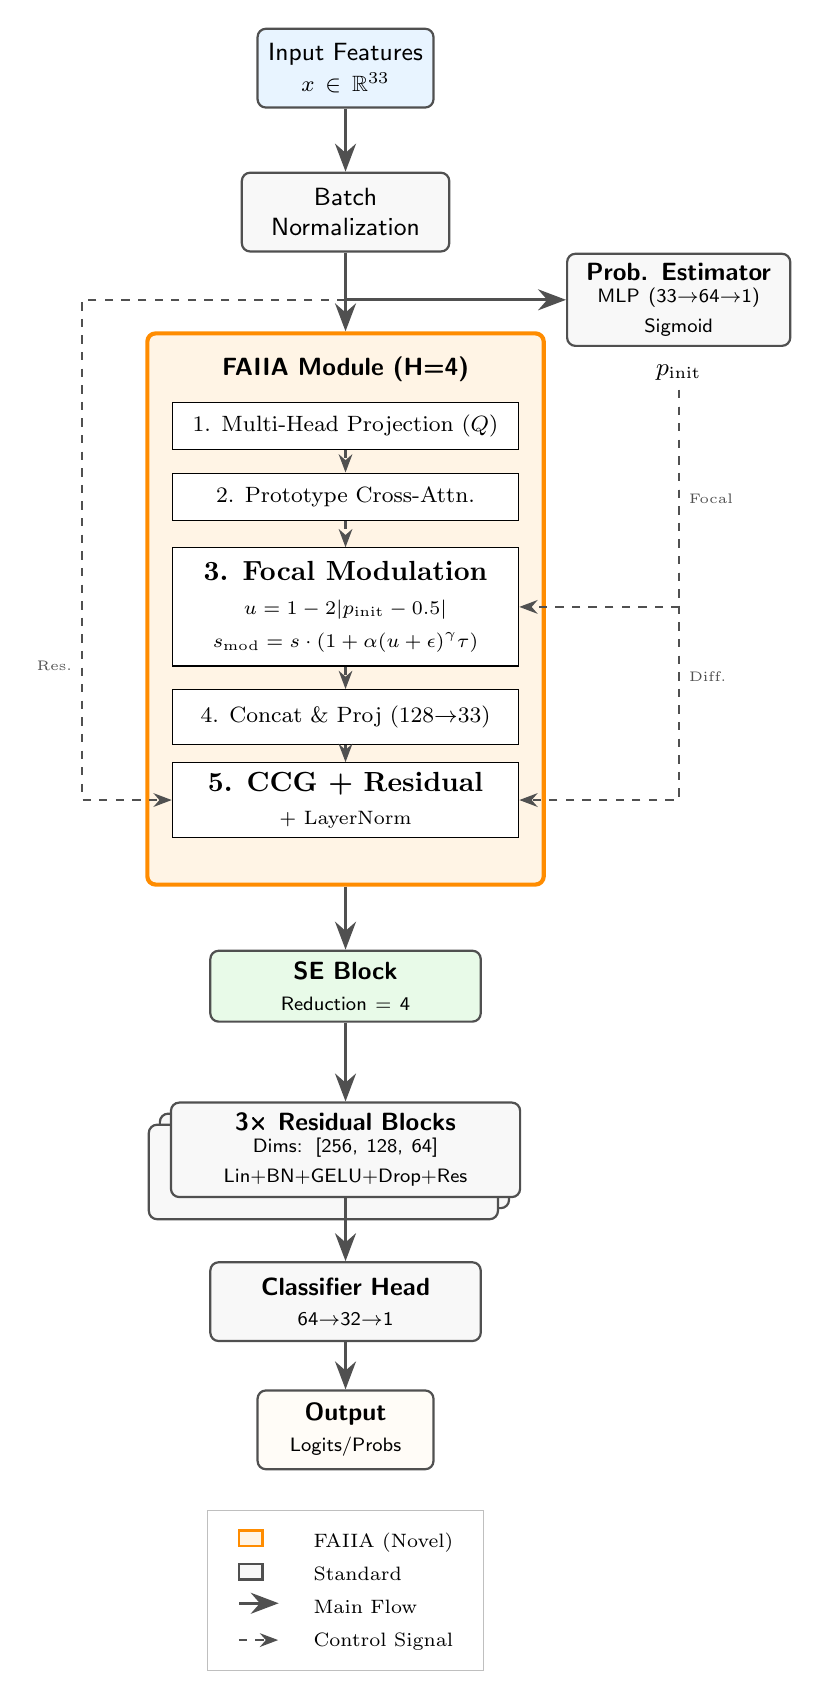
\begin{tikzpicture}[node distance=0.8cm and 1.2cm, >=stealth]

    % --- 1. Input Layer ---
    \node [input] (in) {Input Features \\ \footnotesize $x \in \mathbb{R}^{33}$};
    \node [standard, below=of in] (bn) {Batch \\ Normalization};
    \draw [main_arrow] (in) -- (bn);

    % --- 2. Main Path Split ---
    \coordinate (split) at ($(bn.south) + (0,-0.6)$);
    \draw [line width=1.2pt, color=darkgray] (bn.south) -- (split);

    % Auxiliary Path (Prob. Estimator)
    \node [standard, right=2.8cm of split, text width=2.6cm, anchor=west] (prob) {
        \textbf{Prob. Estimator} \\
        \scriptsize MLP (33$\to$64$\to$1) \\
        \scriptsize Sigmoid
    };
    \node [below=0.1cm of prob, font=\small] (pinit) {$p_{\text{init}}$};
    \draw [main_arrow] (split) -- (prob.west);

    % Main Path (FAIIA Module)
    \node [novel, below=0.4cm of split, minimum height=7.0cm, text width=4.8cm] (faiia_box) {};
    \draw [main_arrow] (split) -- (faiia_box.north);

    % --- 3. FAIIA Internal Detail ---
    \node [anchor=north, font=\sffamily\bfseries\small, yshift=-0.2cm] at (faiia_box.north) {FAIIA Module (H=4)};
    
    \node [rectangle, draw, fill=white, minimum width=4.4cm, minimum height=0.6cm] (heads) at ([yshift=-1.2cm]faiia_box.north) {
        \footnotesize 1. Multi-Head Projection ($Q$)
    };
    
    \node [rectangle, draw, fill=white, minimum width=4.4cm, minimum height=0.6cm] (proto) at ([yshift=-2.1cm]faiia_box.north) {
        \footnotesize 2. Prototype Cross-Attn.
    };
    
    \node [rectangle, draw, fill=white, minimum width=4.4cm, minimum height=1.5cm, align=center] (focal) at ([yshift=-3.5cm]faiia_box.north) {
        \textbf{3. Focal Modulation} \\
        \scriptsize $u = 1 - 2|p_{\text{init}} - 0.5|$ \\
        \scriptsize $s_{\text{mod}} = s \cdot (1 + \alpha(u+\epsilon)^\gamma\tau)$
    };
    
    \node [rectangle, draw, fill=white, minimum width=4.4cm, minimum height=0.7cm] (concat) at ([yshift=-4.9cm]faiia_box.north) {
        \footnotesize 4. Concat \& Proj (128$\to$33)
    };
    
    \node [rectangle, draw, fill=white, minimum width=4.4cm, minimum height=0.9cm, align=center] (ccg) at ([yshift=1.1cm]faiia_box.south) {
        \textbf{5. CCG + Residual} \\
        \scriptsize + LayerNorm
    };

    % Internal Flow Arrows
    \draw [aux_arrow, dashed] (heads) -- (proto);
    \draw [aux_arrow, dashed] (proto) -- (focal);
    \draw [aux_arrow, dashed] (focal) -- (concat);
    \draw [aux_arrow, dashed] (concat) -- (ccg);

    % Focal logic dependency
    \draw [aux_arrow] (pinit.south) |- (focal.east) node[pos=0.25, right, font=\tiny] {Focal};
    
    % CCG dependency
    \draw [aux_arrow] (pinit.south) |- (ccg.east) node[pos=0.35, right, font=\tiny] {Diff.};
    
    % Residual path - routed around left side
    \coordinate (res_left) at ($(faiia_box.west) + (-0.8, 0)$);
    \draw [aux_arrow] (split) -| (res_left) |- (ccg.west) node[pos=0.15, left, font=\tiny] {Res.};
 
    % --- 4. SE Block ---
    \node [post, below=of faiia_box, text width=3.2cm, minimum height=0.9cm] (se) {
        \textbf{SE Block} \\
        \scriptsize Reduction = 4
    };
    \draw [main_arrow] (faiia_box.south) -- (se);

    % --- 5. Residual Blocks (Stacked Representation) ---
    \node [standard, below=1.0cm of se, text width=4.2cm, minimum height=1.2cm] (deep) {
        \textbf{3× Residual Blocks} \\
        \scriptsize Dims: [256, 128, 64] \\
        \scriptsize Lin+BN+GELU+Drop+Res
    };

    % Visual stack effect
    \begin{scope}[on background layer]
        \node [standard, anchor=north west, text width=4.2cm, minimum height=1.2cm] 
            at ($(deep.north west)+(-4pt,-4pt)$) {};
        \node [standard, anchor=north west, text width=4.2cm, minimum height=1.2cm] 
            at ($(deep.north west)+(-8pt,-8pt)$) {};
    \end{scope}

    \draw [main_arrow] (se.south) -- (deep.north);

    % --- 6. Classifier Head ---
    \node [standard, below=0.8cm of deep, text width=3.2cm] (classifier) {
        \textbf{Classifier Head} \\
        \scriptsize 64$\to$32$\to$1
    };
    \draw [main_arrow] (deep.south) -- (classifier.north);

    % --- 7. Output ---
    \node [input, below=0.6cm of classifier, fill=coreorange!30] (out) {
        \textbf{Output} \\
        \scriptsize Logits/Probs
    };
    \draw [main_arrow] (classifier.south) -- (out.north);

    % --- Legend ---
    \node [draw=gray!50, rounded corners=0, inner sep=5pt, below=0.5cm of out] (legend) {
        \begin{tabular}{ll}
            \tikz\draw[thick, accentorange, fill=coreorange] (0,0) rectangle (0.3,0.2); & \scriptsize FAIIA (Novel) \\
            \tikz\draw[thick, darkgray, fill=standardgray] (0,0) rectangle (0.3,0.2); & \scriptsize Standard \\
            \tikz\draw[main_arrow] (0,0) -- (0.5,0); & \scriptsize Main Flow \\
            \tikz\draw[aux_arrow] (0,0) -- (0.5,0); & \scriptsize Control Signal
        \end{tabular}
    };

\end{tikzpicture}

\end{document}